\documentclass{beamer}
\usepackage[utf8]{inputenc}

\usetheme{Madrid}
\usecolortheme{default}
\usepackage{amsmath,amssymb,amsfonts,amsthm}
\usepackage{txfonts}
\usepackage{tkz-euclide}
\usepackage{listings}
\usepackage{adjustbox}
\usepackage{array}
\usepackage{tabularx}
\usepackage{gvv}
\usepackage{lmodern}
\usepackage{circuitikz}
\usepackage{tikz}
\usepackage{graphicx}

\setbeamertemplate{page number in head/foot}[totalframenumber]

\usepackage{tcolorbox}
\tcbuselibrary{minted,breakable,xparse,skins}



\definecolor{bg}{gray}{0.95}
\DeclareTCBListing{mintedbox}{O{}m!O{}}{%
  breakable=true,
  listing engine=minted,
  listing only,
  minted language=#2,
  minted style=default,
  minted options={%
    linenos,
    gobble=0,
    breaklines=true,
    breakafter=,,
    fontsize=\small,
    numbersep=8pt,
    #1},
  boxsep=0pt,
  left skip=0pt,
  right skip=0pt,
  left=25pt,
  right=0pt,
  top=3pt,
  bottom=3pt,
  arc=5pt,
  leftrule=0pt,
  rightrule=0pt,
  bottomrule=2pt,
  toprule=2pt,
  colback=bg,
  colframe=orange!70,
  enhanced,
  overlay={%
    \begin{tcbclipinterior}
    \fill[orange!20!white] (frame.south west) rectangle ([xshift=20pt]frame.north west);
    \end{tcbclipinterior}},
  #3,
}
\lstset{
    language=C,
    basicstyle=\ttfamily\small,
    keywordstyle=\color{blue},
    stringstyle=\color{orange},
    commentstyle=\color{green!60!black},
    numbers=left,
    numberstyle=\tiny\color{gray},
    breaklines=true,
    showstringspaces=false,
}
\title{1.9.34}
\date{4th September, 2025}
\author{EE25BTECH11018 - Darisy Sreetej}

\begin{document}

\frame{\titlepage}
\begin{frame}{Question}
Find the distance of the point \brak{-6,8} from the origin.
\end{frame}

\begin{frame}{allowframebreaks}
\frametitle{Equation}
The distance of the point from the origin is the length of its position vector $\vec{P}$. The formula is given as 
\begin{align}
\norm{\vec{P}} = \sqrt{\vec{P}^\top \vec{P}} \label{eq:1}
\end{align}
\end{frame}

\begin{frame}{Solution}
\begin{align*}
    \vec{P}^\top = \myvec{-6 & 8}
\end{align*}

From \ref{eq:1}, we have
\begin{align}
    \vec{P}^\top \vec{P} &= \myvec{-6 & 8} \myvec{-6 \\ 8} \\
    &= \brak{-6}\brak{-6} + \brak{8}\brak{8} \\
    &= 36 + 64 \\
    &= 100
\end{align}
\end{frame}

\begin{frame}{allowframebreaks}
\frametitle{Solution}
\begin{align*}
    \text{Distance} = \norm{\vec{P}} = \sqrt{\vec{P}^\top \vec{P}} = \sqrt{100} = 10
\end{align*}

$\therefore$ The distance of the point \brak{-6, 8} from the origin is \textbf{10 units}.
\end{frame}

\begin{frame}{Plot-Graph}
    \begin{figure}
        \centering
        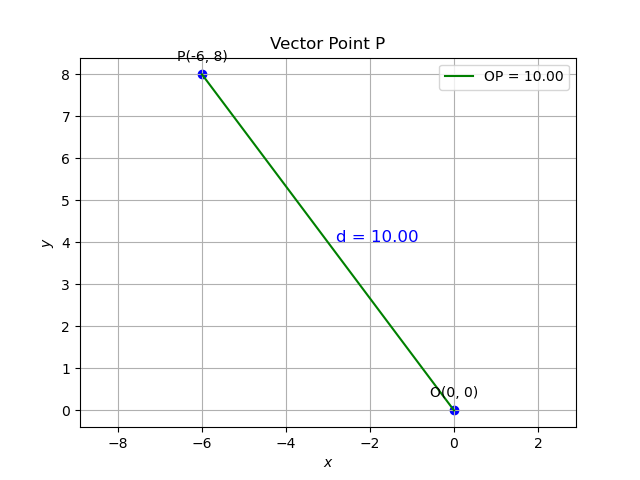
\includegraphics[width=0.5\columnwidth]{../figs/fig.png}
        \caption{Point P\brak{-6,8}}
        \label{fig:fig}
    \end{figure}
\end{frame}

\end{document}